
\documentclass[ebook,12pt,twoside,openright,extrafontsizes,final]{memoir}
\usepackage{fontspec}
\usepackage{lettrine}
\usepackage{longtable}
\usepackage{graphicx}
\graphicspath{ {./} }

\setsecnumdepth{chapter}
\setmainfont[  
    Numbers={OldStyle},
    Ligatures={Rare,Historic}
    % ,ItalicFeatures={Colour=990000}
]{EBGaramond}

\medievalpage
\checkandfixthelayout

\nouppercaseheads

\begin{document}
\frontmatter
\title{The Game of Triumphs}
\author{Michael Shirk}
\date{MMXIX}
\maketitle

\tableofcontents


Preface
Brief history,
explanation of teh goals of the book.

Read the Prelimiaries. 
Table of num of players x complexity

\mainmatter

\chapter{Preliminaries}
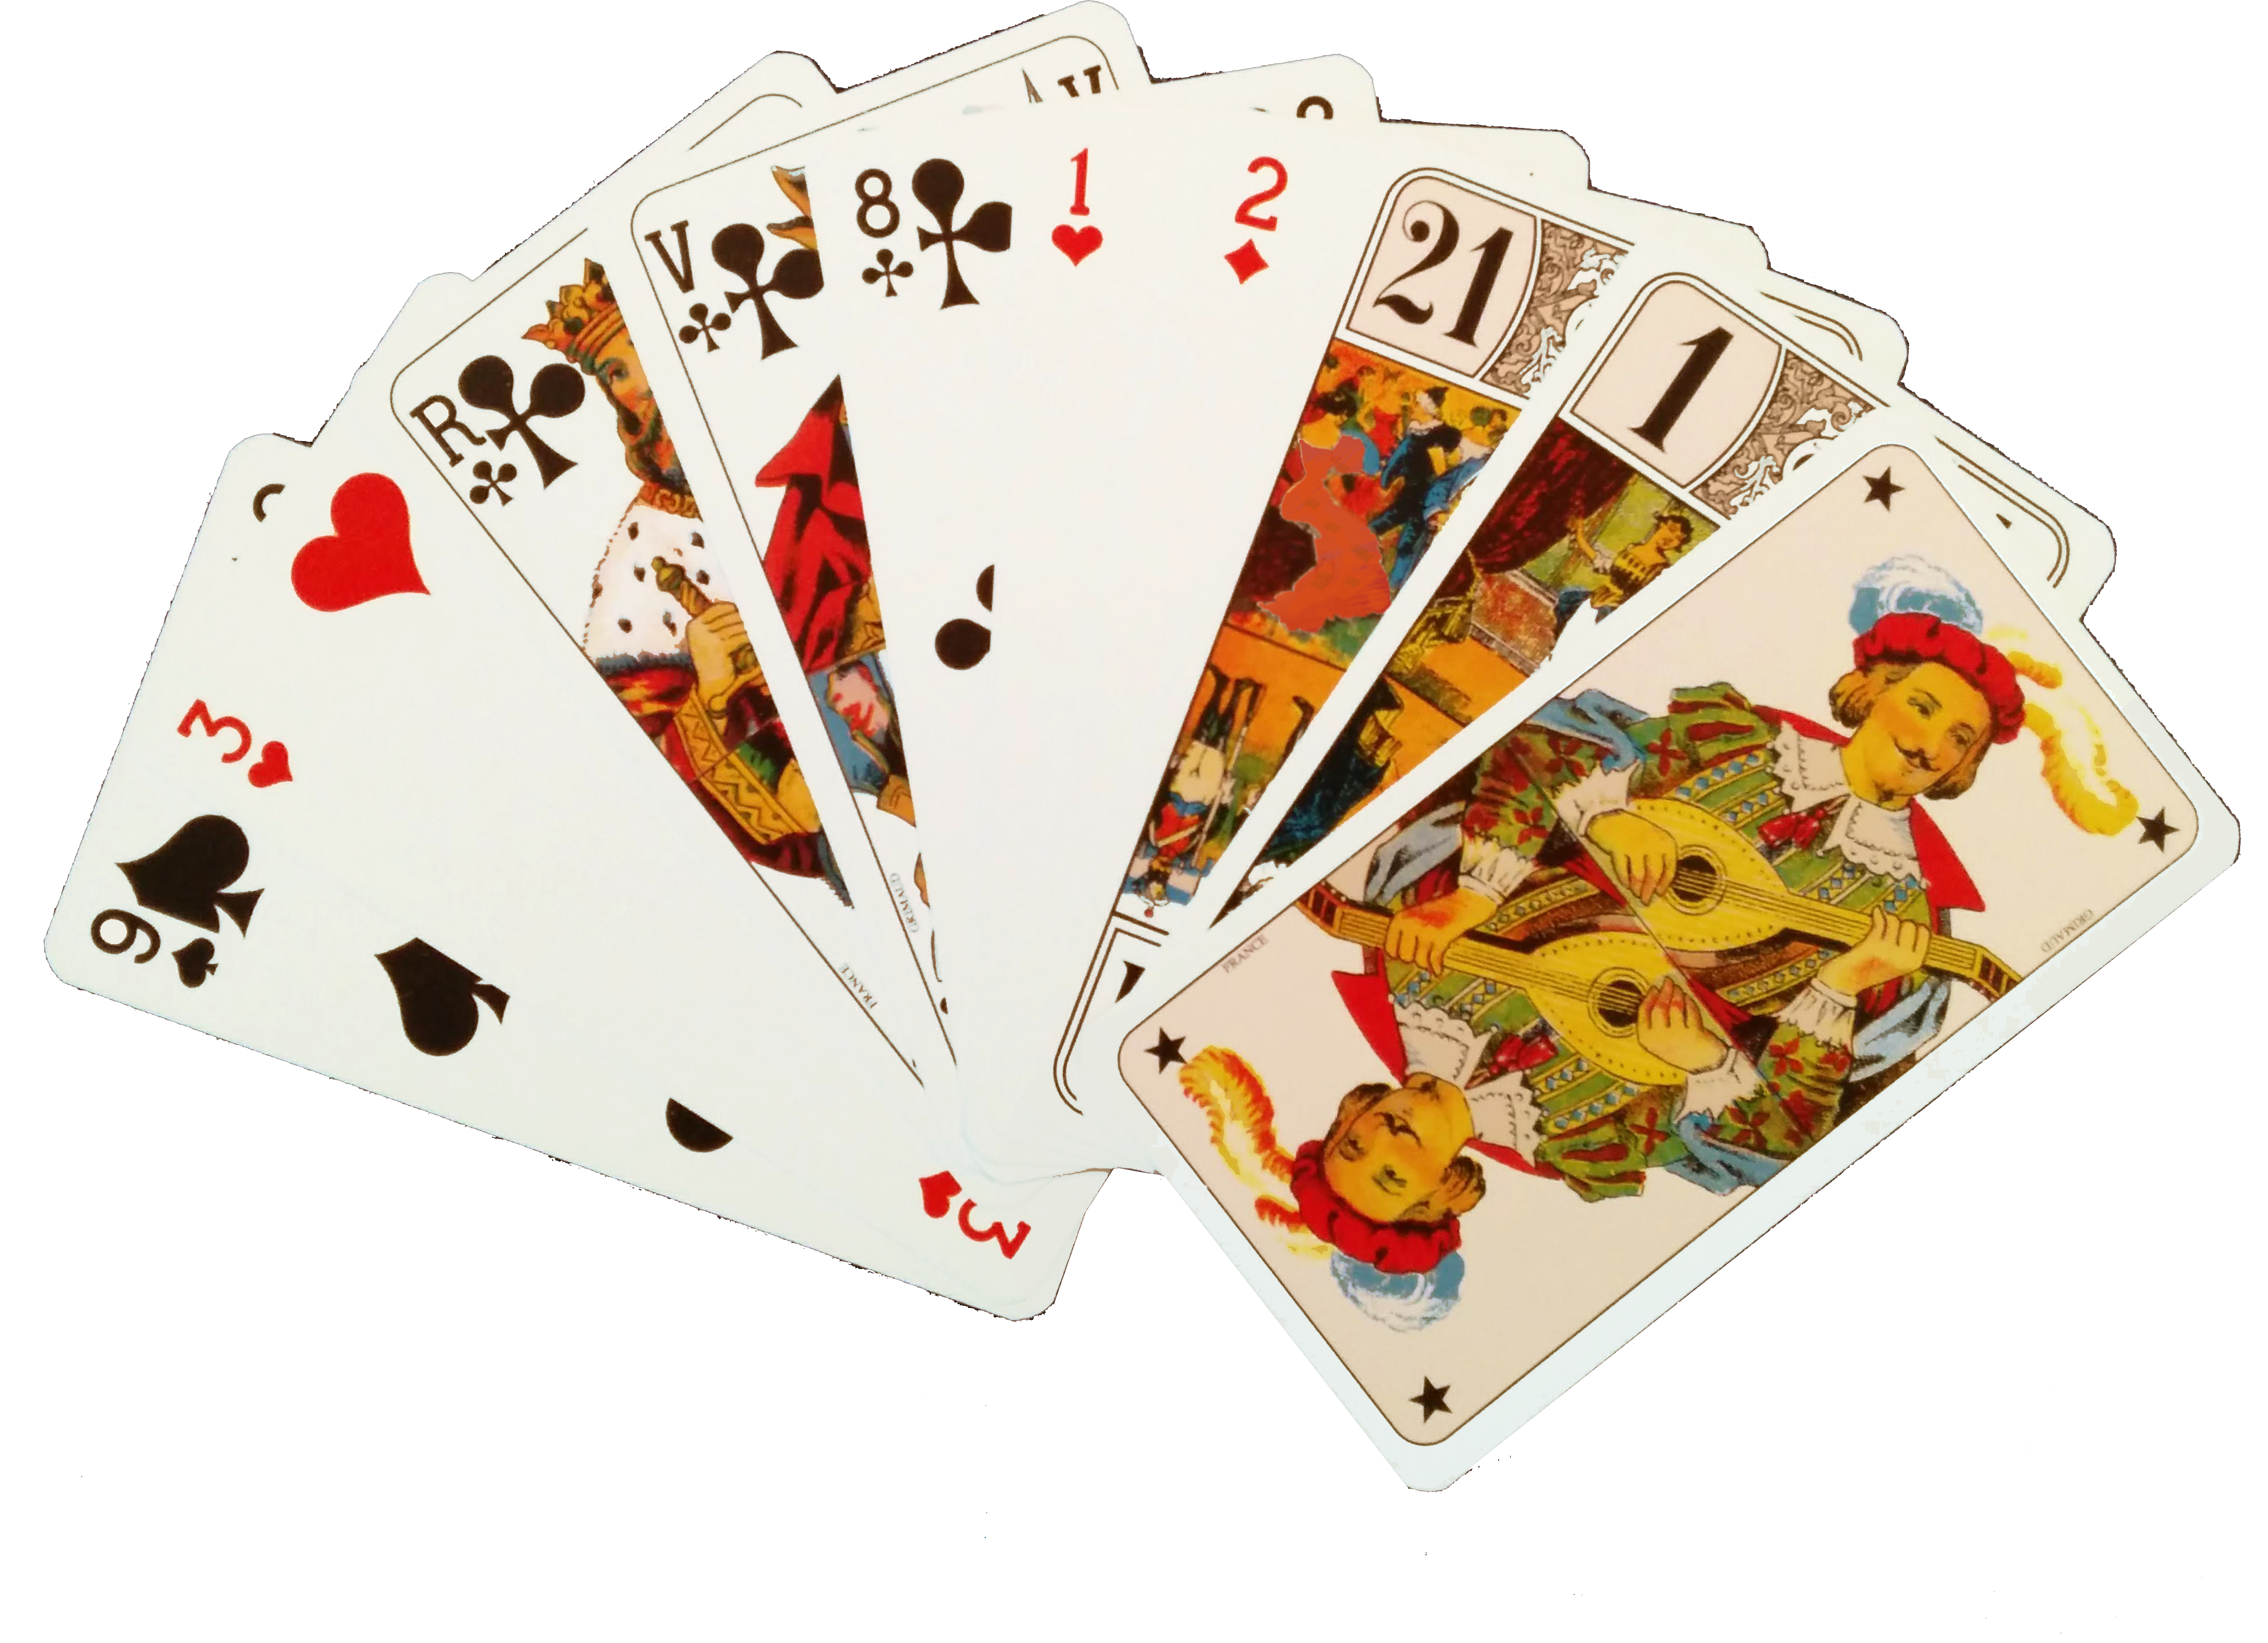
\includegraphics[width=\textwidth]{french}
\section{The Deck}
\lettrine{T}{he} Tarot deck is comprised of the four usual suits – but with four, rather
than three Court Cards – and a fifth suit that serves as permanent Trumps.
The first Tarot decks used the same suits that are still used in Italy:
Cups, Coins, Swords, and Batons.\footnote{Current Italian-suited decks include:
the Tarot de Marseille, the Swiss IJJ, and the Tarocco Piemontese.}  In fact,
the Tarot deck was originaly simply the addition of a fifth suit, consisting 
of allegorical subjects, to the ordinary deck of cards.  In the 18th century, 
cardmakers in the German-speaking world began producing Tarot decks with the French suits
of Hearts, Spades, Clubs and Diamonds, and with animals or scenes on the
trump suit rather than the traditional subjects. These French-suited
Tarot decks are now used in France, Germany, Denmark, parts of Switzerland, 
and all the countries of the former Austro-Hungarian Empire.\footnote{These
decks include the Tarot Nouveau, the Industrie und Glück, and the Adler-Cego.}
The Italian suited decks persist only in Italy, parts of Switzerland, and Sicily.

The original deck contained 78 cards: 14 cards each in the ordinary suits, 
21 Trumps, and a special card called ‘The Fool’, or later ‘The Excuse.’
This deck is still used in France and Denmark.  In other areas, however,
the deck is reduced in size by omitting the lower ranking pips in the ordinary
suits. In Austria and countries influenced by it, the Excuse became the highest
Trump, and the deck was reduced to 54 cards: 8 cards per suit (four Court Cards 
and four pips) and the 22 Trumps.

A peculiarity of the deck which goes back even before Tarot to the introduction
of playing cards into Europe, and persists to the present in almost all Tarot
games, is that the pips in the Red or Round suits (Heart and Diamonds, or Cups
and Coins) rank upside down.  Those suits rank, from high to low: King, Queen,
Knight, Jack, 1, 2, 3, 4, 5, 6, 7, 8, 9, 10.

  

[name the courts, indexes, italian and french. Table]

\section{Order of Play}
Unlike most games in the English-speaking world, Tarot games are almost always
played counterclockwise.  The order of play, of course, makes little 
difference; but it is a feature of Italian card games that Tarot has always 
carried with it.

\section{The Deal and Discard}
The cards are usually dealt in groups, rather than singly. This \emph{can} make
a difference; in some games it is the convention (though not the rule) not to
shuffle the deck between deals, but only to cut it. This is supposed to lead
to more interesting hands.

The cards should not be touched until the deal is complete, and then counted.
This way if any mistake was made during dealing, it can be corrected without
having to redeal.

Tarot cards are usually larger than Poker cards, and there are usually more of 
them in hand.  It can be easier to pick the cards up on or two at a time and 
add them to your hand, rather than picking up your entire hand at once and sorting
it in place.  If you're playing with a deck without indices, or with the full 
deck of 78, it might well be impractical to fan your cards out so that you can 
see them all, as you might be used to in other games. Rather, glance through to
get a general idea of your hand, and then fan out only the part that is relevant
to each play. Note also that cards in the Marseille tradition have roman numeral
indexes on the sides, rather than in the corners.

There will be a few cards left over after the deal.  In older games these belong
to the Dealer; in newer ones they will go to the eventual Declarer. That
individual will pick them up and add them to their hand, and then discard 
the same number of cards. The cards in the discard will count for them in the 
end, thus it can sometimes be advantageous to discard point cards.

The usual rules of discarding are that one may \emph{never} discard Honours (Kings, the I and 
XXI of Trumps, and the ’Scuse), and one may only discard other Trumps if necessary to avoid 
discarding an Honour. 

\section{Bidding}
In Tarot games with bidding, the bids rarely alter the "target" of the play, they way 
they do in Spades or Bridge.  Instead, they alter the \emph{conditions} under which one is
willing to aim for a set target—or, in the Austrian family, what the rules of the game
itself will be.  The eventual winner of the bidding will become the Declarer. She alone
(or, perhaps with a partner) will attempt to win the game she has bid and will score
accordingly.  The other players – the Defenders – will attempt to thwart her.

Bidding is done in one round, and proceeds as follows. The Eldest player (the next in
rotation after the dealer) will bid or pass.  If he bids, the next in rotation may make a
higher bid, or pass.  If she makes a higher bid, it goes back to the previous bidder, 
who may \emph{match} the higher bid - or pass. As soon as one of the first two players has
passed, bidding proceeds between the player who did not pass and the third player.  Said 
another way, bidding is always between two players: either the first two who who have not
passed, or between the one who has not passed yet and the next in rotation. 

One you have passed, you may not reenter the bidding.


\section{Tricks}
Tarot games are all Trick-taking games. The most prestigious game of this family
in the English speaking world is Bridge; perhaps the most common, due
to its ubiquity on the Windows operating system, is Hearts.

A Trick consists of every player playing one card to the center of the table. 
The first player to play is said to lead to the trick: the suit of the card
they play is called the suit led.  Every other player in rotation must, if
they can, play a card of the same suit from their hand.  If they have no cards
of the suit led, they must play a card from the Trump suit.  If they have no 
remaining trumps either, they may play any card.  The highest trump, or (if 
no trumps were played) the highest card of the suit led wins. The player who
played it collects the cards and places them facedown in a pile in front of
him, and then leads to the next trick.

In the older forms of the game, the ’Scuse is the exception to the rules of
following suit.  The holder of the ’Scuse may play it at any point. It never
wins a trick - but it isn’t lost: the player of the ’Scuse, after showing it,
takes it back and adds it to his trick pile, and gives a worthless card in
exchange for it.  If the player never takes a trick, the ’Scuse is forfeited
to the person who won the trick to which it was played.  The ’Scuse is also
forfeited to the winner of the trick if played to the last trick.  If the 
’Scuse is led to a trick, the next player may play anything, and their card
counts as the lead.

In the Austrian games, the ’Scuse is simply the XXII of Trumps.

Tarot games are furthermore \emph{Point Trick} games.  Not only do the tricks
have value, but certain cards carry a value in and of themselves.
These cards are the Court Cards, and the Trull: the I and XXI of Trumps,
and the ’Scuse.

Unless otherwise specified, the eldest player will always lead to the first
trick.


\section{Counting Points}
The original method of counting points after the hand, which is still the easiest
to start with, is to count the points for all Court Cards and for the Trull (the I
and XXI of Trumps and the ’Scuse), and then to add one point per trick taken.  In 
fact, in almost all variations the number of cards constituting the ‘trick’ is 
conventionalized, regardless of how many people are playing. Thus, each game will 
specify that the cards are counted ‘in twos,’ ‘in threes,’ or ‘in fours.’

\begin{table}[]
\centering
\begin{tabular}{lc}
\multicolumn{1}{c}{\textbf{Card}} & \textbf{Value} \\
I, XXI, \& ’Scuse & 4 each\\
Kings & 4 each \\
Queens & 3 each\\
Knights & 2 each\\
Jacks & 1 each
\end{tabular}
\end{table}

In other descriptions of Tarot games other counting methods will be described. Although
they may seem rather different, they add up to the same values.

\chapter{“Basic Tarot”}
This game forms the core of all following games. It has been played most 
places where Tarot has permiated, under various names: in Switzerland
it is played as \emph{Troccas}, in Lombardy as \emph{Tarocchi}, and in Piedmont
as \emph{Tarocchi} or \emph{Scarto}, with slight differences.

\medskip
\lettrine{A}{ game} is made up of as many deals as their are players.  After the 
three or four deals of the game, whoever has the lowest score pays a small stake 
to the others, such as buying the next round of drinks.

Played with a 78 card deck. The ’Scuse serves as Excuse.

\section{Three Player}
The Dealer deals 25 cards to each player in batches of 5.  She then takes the
remaining 3 cards into her own hand and discards three.
At the end of the hand, each player counts their cards in groups of 3.  There
are 78 points total in the deck.  Each player's score is recorded as the 
difference between the card points they took and 26.

\section{Four Player}
The players sitting opposite each other are partners, and score as a team.
The Dealer deals 19 cards to each player.  He then takes the remaining 2 into 
his own hand and discards two.
At the end of the hand, each team counts their cards in groups of 4. (The 
Dealer’s discard counts as a full trick.)  There are 72 points total in the 
deck.  Each player's score is recorded as the difference between the card 
points they took and 36.


\chapter{Großtarock}
The classic form of the game, played for over a hundred years in France, Germany, 
Italy, and Austria came to be known as Großtarock in German-speaking lands, to contrast
it with the newer game played with only 54 cards. It is still played in Denmark, and 
similar games are played in northern Italy as \emph{Mitigati.}

\section{Three or Four Player}
\lettrine{T}{hree} players are active at a time. If four participate, the player opposite
the dealer takes no part in a given hand.  A game may consist of as many hands as desired,
as long as each player is allowed to deal an equal number of times.


The Dealer deals 25 cards to each player in batches of 5.  She then takes the
remaining 3 cards into her own hand and discards three.  The usual restrictions apply. 
Furthermore, no card that would otherwise be part of one of the following Declarations may 
be discarded.

\subsection{Declarations}
Starting with the Dealer and going in order, each player must make any of the following 
Declarations of card combinations they hold.

\begin{longtable}[c]{lp{3in}}
\multicolumn{1}{c}{} & \multicolumn{1}{c}{\textit{Description}} \\
\endfirsthead
\endhead
\textbf{Trumps} & ‘Ten Trumps’ is worth \textbf{10} points; more may be declared for 
\textbf{5} more each. (\emph{E.g.}, ‘Eleven Trumps’ is \textbf{15}, ‘Twelve Trumps’ is 
\textbf{20}, \emph{\&c.})  For the purposes of the declaration, the ’Scuse counts as
a trump. It must be stated whether ‘with’ or ‘without’ the Pagat. \\
\textbf{Matadors} & ‘Three Matadors’ consists of the three cards of the Trull, for 
\textbf{10} points. ‘Four Matadors’ adds the XX of Trumps for \textbf{15}, ‘Five 
Matadors’ the XX and XIX for \textbf{20}, \emph{\&c.} \\
\textbf{Cavalry} & A ‘Cavalry’ is a set of all four Court Cards in one suit for \textbf{10}; 
a ‘Half Cavalry’ is any three Court Cards in one suit plus the ’Scuse for \textbf{5}, and 
an ‘Abundant Cavalry’ is all four Courts plus the ’Scuse for \textbf{15}. The suit (and 
missing card) must be named. \\
\textbf{Kings} & ‘Kings’ is all four Kings for \textbf{10}; ‘Half Kings’ is any three plus 
the ’Scuse for \textbf{5}, and ‘Abundant Kings’ is all four Kings plus the ’Scuse for 
\textbf{15}. The missing suit (for Half) must be named.
\end{longtable}

\subsection{Play}
Eldest leads to the first Trick. The ’Scuse serves as Excuse. If played to any of the last
three tricks it is lost to the winner of the trick.

A player who loses a King or the Pagat to another player before the final trick pays 
\textbf{5} points to each of them.

At the end of the hand, one of the following conditions will be met:
\begin{longtable}[c]{lp{3in}}
\multicolumn{1}{c}{} & \multicolumn{1}{c}{\textit{Description}} \\
\endfirsthead
\endhead
\textbf{Tout} & One player has taken all tricks.  He is payed \textbf{85} by each other 
    player. \\
\textbf{Nill} & Exactly one player only has taken no tricks. She is payed \textbf{25} by 
    each other player. Ultimos and card points are not scored, but Failed Ultimos are.\\
\textbf{Ultimo} & One player has taken the last trick with the Pagat or with a King. He is 
    payed \textbf{45} for the Pagat, or \textbf{40} for the King, by each other player. 
    Other players may score a Failed Ultimo at the same time. \\
\textbf{Failed Ultimo} & Any player who plays a Pagat or a King to the last trick, but 
    does not win the trick. She pays \textbf{45} for the lost Pagat or \textbf{40} for 
    the lost King to each other player.\\
\textbf{Last Trick} & If none of the above has occured, the player who wins the last trick.
    He is payed \textbf{20} by each other player. \\
\end{longtable}

Finally, each player counts the card points they took.  The total should always come to 
\textbf{78}

\subsection{Scoring with Paper}
For the above declarations, bonuses during play, and final outcome after the last trick,
the value noted is recorded as positive for a player who ‘is payed’ or as negative for
the player who ‘pays’.  Only the subject player receives a score. For example, if a player
declares ‘Ten Trumps’, he is payed 10: so \textbf{10} is added to his score.  If a player
loses a King on the last trick for a Failed Ultimo, she pays 40: so \textbf{-40} is added
to her score.

Finally, the positive or negative difference from \textbf{26} each player took in card
points is added to the score (unless a Nill occured)

\subsection{Scoring with Counters and Pots}
The use of counters and pots for scoring is more traditional, and makes the Ultimos much
more exciting.

Each player begins with a set of counters: 20 units of \textbf{5} and 10 units each of 
\textbf{20} and \textbf{50} should be sufficient. Ideally each player’s counters are 
a different color, so that it's easy to see who’s ahead and who’s behind.

There are two Ultimo Pots, one each for the Pagat and for a King. These might be a saucer
for the Pagat and a small bowl in the center for Kings.

Whenever either pot is empty, including at the start of the game, every player (including
the fourth, if four play) contribute \textbf{20} points to it as a foundation.

After dealing and discarding, the Dealer contributes \textbf{5} to each pot. Afterwords she
moves the pots between her and eldest, to indicate that the discard is complete.

Payments for declarations or bonuses are made as described in the main rules. In addition,
a player who loses a King or the Pagat before the last trick also adds \textit{5} to the
appropriate pot. 

A winner of a Tout also receives the contents of both pots; a winner of an Ultimo receives
the contents of the appropriate pot.  A player who fails an Ultimo doubles the appropriate
pot.  If a failed Ultimo and an Ultimo or Tout concern the same pot, first the value is
counted and given to the winner; then the same amount is contributed back in by the loser.

Unless a Nill occured, each player then counts their card points, and pays the next dealer
according to the following table:

\begin{center}
\begin{tabular}{cl}
\textbf{9-13}  & pay dealer 15\\
\textbf{14-18} & pay dealer 10\\
\textbf{19-23} & pay dealer 5 \\
\textbf{24-28} & no payment\\
\textbf{29-33} & receive 5 from dealer\\
\textbf{34-38} & receive 10 from dealer\\
\textbf{39-43} & receive 15 from dealer
\end{tabular}
\end{center}

At the end of play, the contents of both pots are distrubted equally among the players.



\section{Two Player}
\lettrine{A}{ll} as above, except:
Two hands of 25 are dealt, the dealer taking 3 extra cards.  The remaining 25 cards, called
the \emph{Mort} are set aside unused for that hand.

Players accumulate the points for Declarations, card points, and bonuses as above. 

There is no award for {Tout} or {Nill}. The payents for Ultimos and the last trick are 
reduced to \textbf{15} for the Pagat, \textbf{10} for a King, and \textbf{5} for the
Last Trick

The Score may be kept on paper or a Cribbage board.  The first to reach \textbf{100} wins.


\chapter{Tarock-l’Hombre}
(6.7, 7.1)
Droggn?
(8.28) Chambéry?


\chapter{Le Jeu de Tarot}
c. 1900
Petit en dedans (2000)
Mouches
Score of base + dif (no mult) 1977, Grenoble
base of 10 + diff mult OR 
base of 10, 20, 30, 50 no mult


\chapter{Dreiertarock}

\chapter{Strawman}

\chapter{Königrufen}

\chapter{Strategy}

glossary?

\end{document}